\documentclass[UTF8]{article}

\usepackage{ctex}
\usepackage{fancyhdr} %自定义页眉页脚
\usepackage{listings} %source code
\usepackage{tabu}
\usepackage{booktabs}
\usepackage{graphicx}
\usepackage{multirow}
\usepackage[colorlinks,linkcolor=blue]{hyperref}
\usepackage{subfigure}
\usepackage{float}
\begin{document}


\begin{titlepage}
\center{北京理工大学计算机学院2017级}
\vspace{0.5cm}
\center{\huge{《数字逻辑》实验一 实验报告}}
\vspace{0.5cm}
\center{\Huge{可调速循环流水灯}}
\vspace{0.5cm}

\begin{center}
\begin{large}
\begin{tabular}{r c}
小组编号& 44\\
\cline{2-2}\\
\hline
学\qquad 号& 1120173323 \\
\cline{2-2}\\
姓\qquad 名& 王聚海 \\
\cline{2-2}\\
班\qquad 级 & xxxx \\
\cline{2-2}\\
\hline
学\qquad 号& 1120171224 \\
\cline{2-2}\\
姓\qquad 名& 冯开宇 \\
\cline{2-2}\\ 
班\qquad 级 & 07011701 \\
\cline{2-2}\\
\hline
学\qquad 号& 1120172200 \\
\cline{2-2}\\
姓\qquad 名& 刘思雨 \\
\cline{2-2}\\ 
班\qquad 级 & 07011701 \\
\cline{2-2}\\

\end{tabular}
\end{large}
\end{center}
\vfill \hfill
\end{titlepage}
\clearpage


\section{设计题目}

\begin{center}
    
\center{可调速循环流水灯}
\end{center}

\section{设计目的}
\begin{enumerate}
    \item 熟悉一次完整的FPGA开发流程,从新建工程,代码设计,综合实现,管脚约束,下载FPGA程序。
    \item 熟悉Xilinx Vivado开发环境,Verilog语言编程基本框架。
    \item 熟悉EES-338口袋计算机硬件平台。
\end{enumerate}

每次上电,按一下rst复位键,LED0~LED7全亮,按住run键,则流水灯从左向右滚动,滚到最右,自动向左滚,滚到左侧,再向右滚动,周而复始。
在循环流水灯基础上,可以通过设计按键调整LED灯的亮灯时间,实现变速流水灯。


\section{设备器材}
\begin{itemize}
    \item Xilinx Vivado开发环境
    \item EES-338口袋计算机硬件平台,配备 FPGA (XC7A35TCSG324-1C)
\end{itemize}



\section{设计原理与内容}

\begin{itemize}
    \item 状态机图
    \item 模块化思想
    \item 边沿检测
\end{itemize}



\section{设计步骤}
\subsection{描述需求}

led灯一共有9个状态,需要控制状态转换的信号(move)以及使信号有效的使能(run)。速度等级level由btnup btndown分别控制。

\subsection{定义输入与输出}

见图\ref{FIG.1}、\ref{FIG.2}。

\begin{figure}[H]
    \centering
    \subfigure[流水灯输入变量]{
        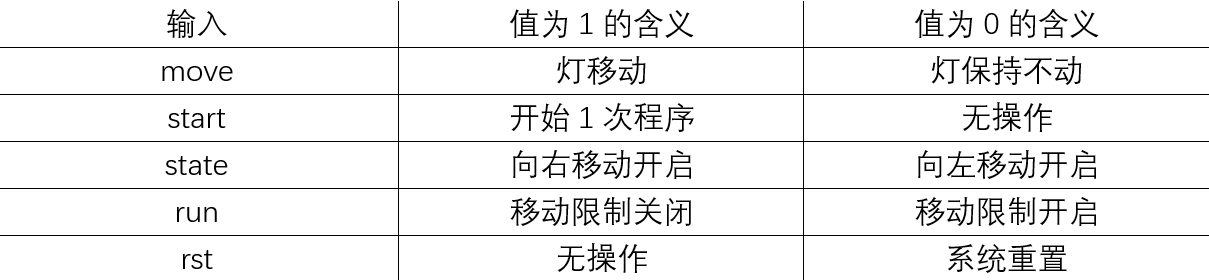
\includegraphics[width=0.45\textwidth]{流水灯控制输入变量.PNG}
        % \caption{流水灯控制输入变量}
        \label{FIG.1}
    }
    \subfigure[流水灯输出变量]{
        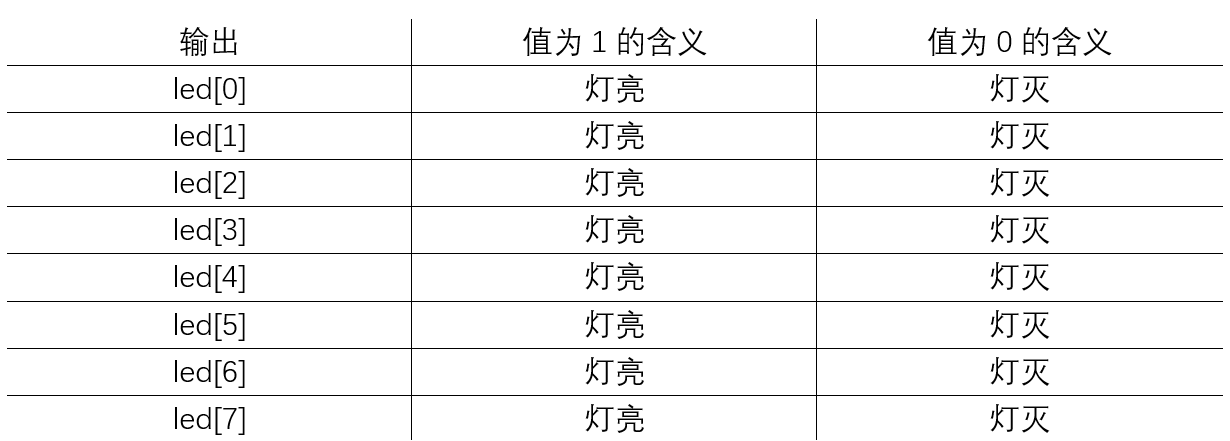
\includegraphics[width=0.45\textwidth]{流水灯输出变量.PNG}
        % \caption{流水灯输出变量}
        \label{FIG.2}
    }
    \caption{流水灯变量分析}
\end{figure}



% GRAGH
\subsection{状态机图}
% GRAGH
见图\ref{FIG.3}、\ref{FIG.4}。

\begin{figure}[H]
    \centering
    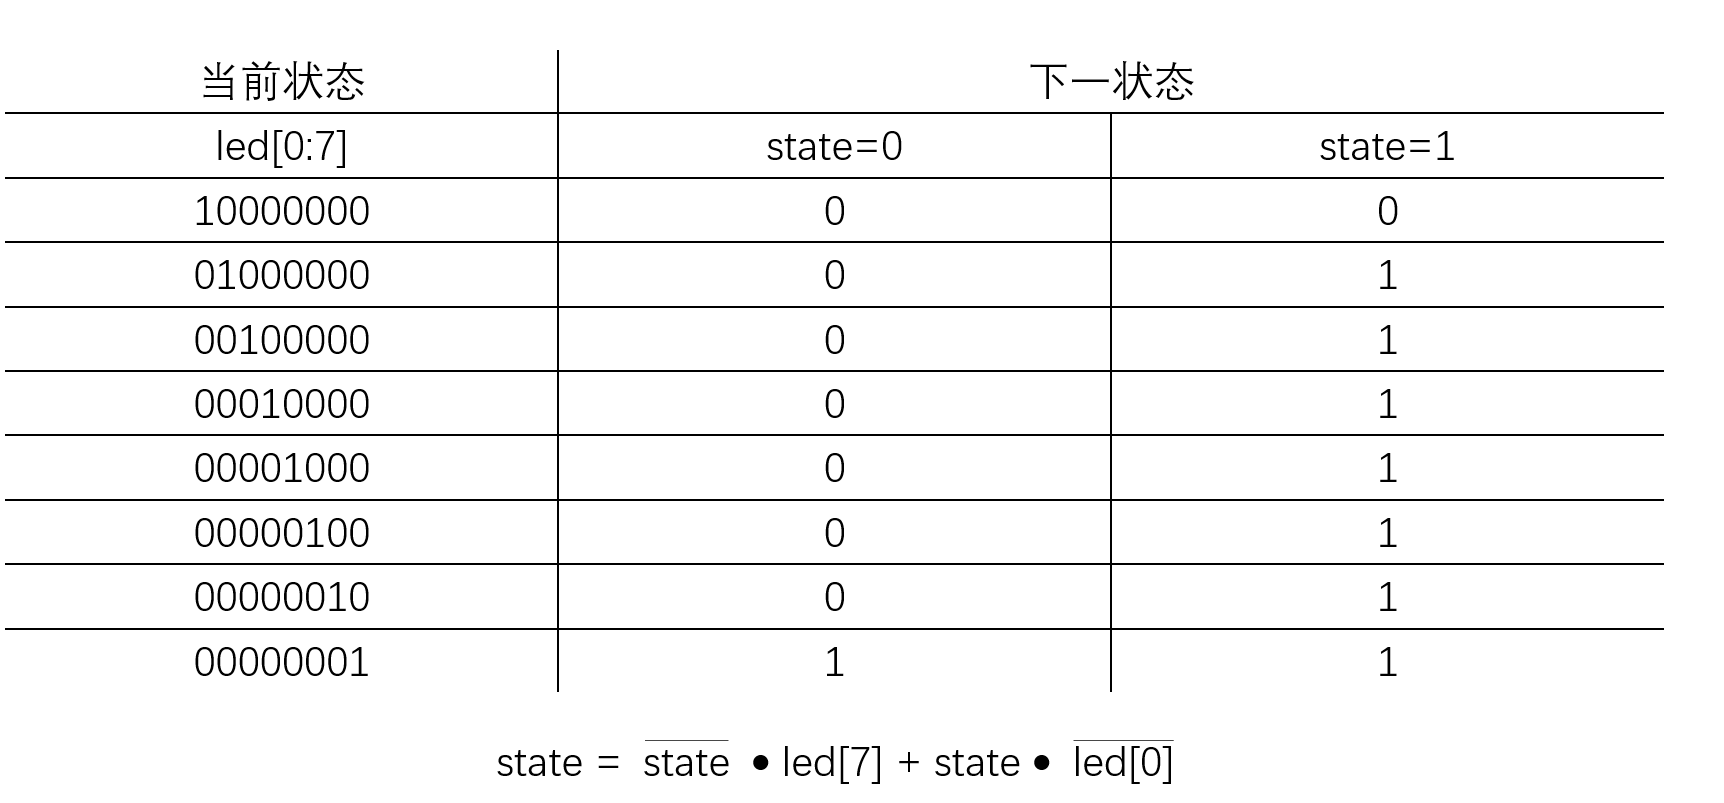
\includegraphics[scale=0.5]{state状态表及布尔表达式.PNG}
    \caption{state状态表及布尔表达式}
    \label{FIG.3}
\end{figure}

\begin{figure}[H]
    \centering
    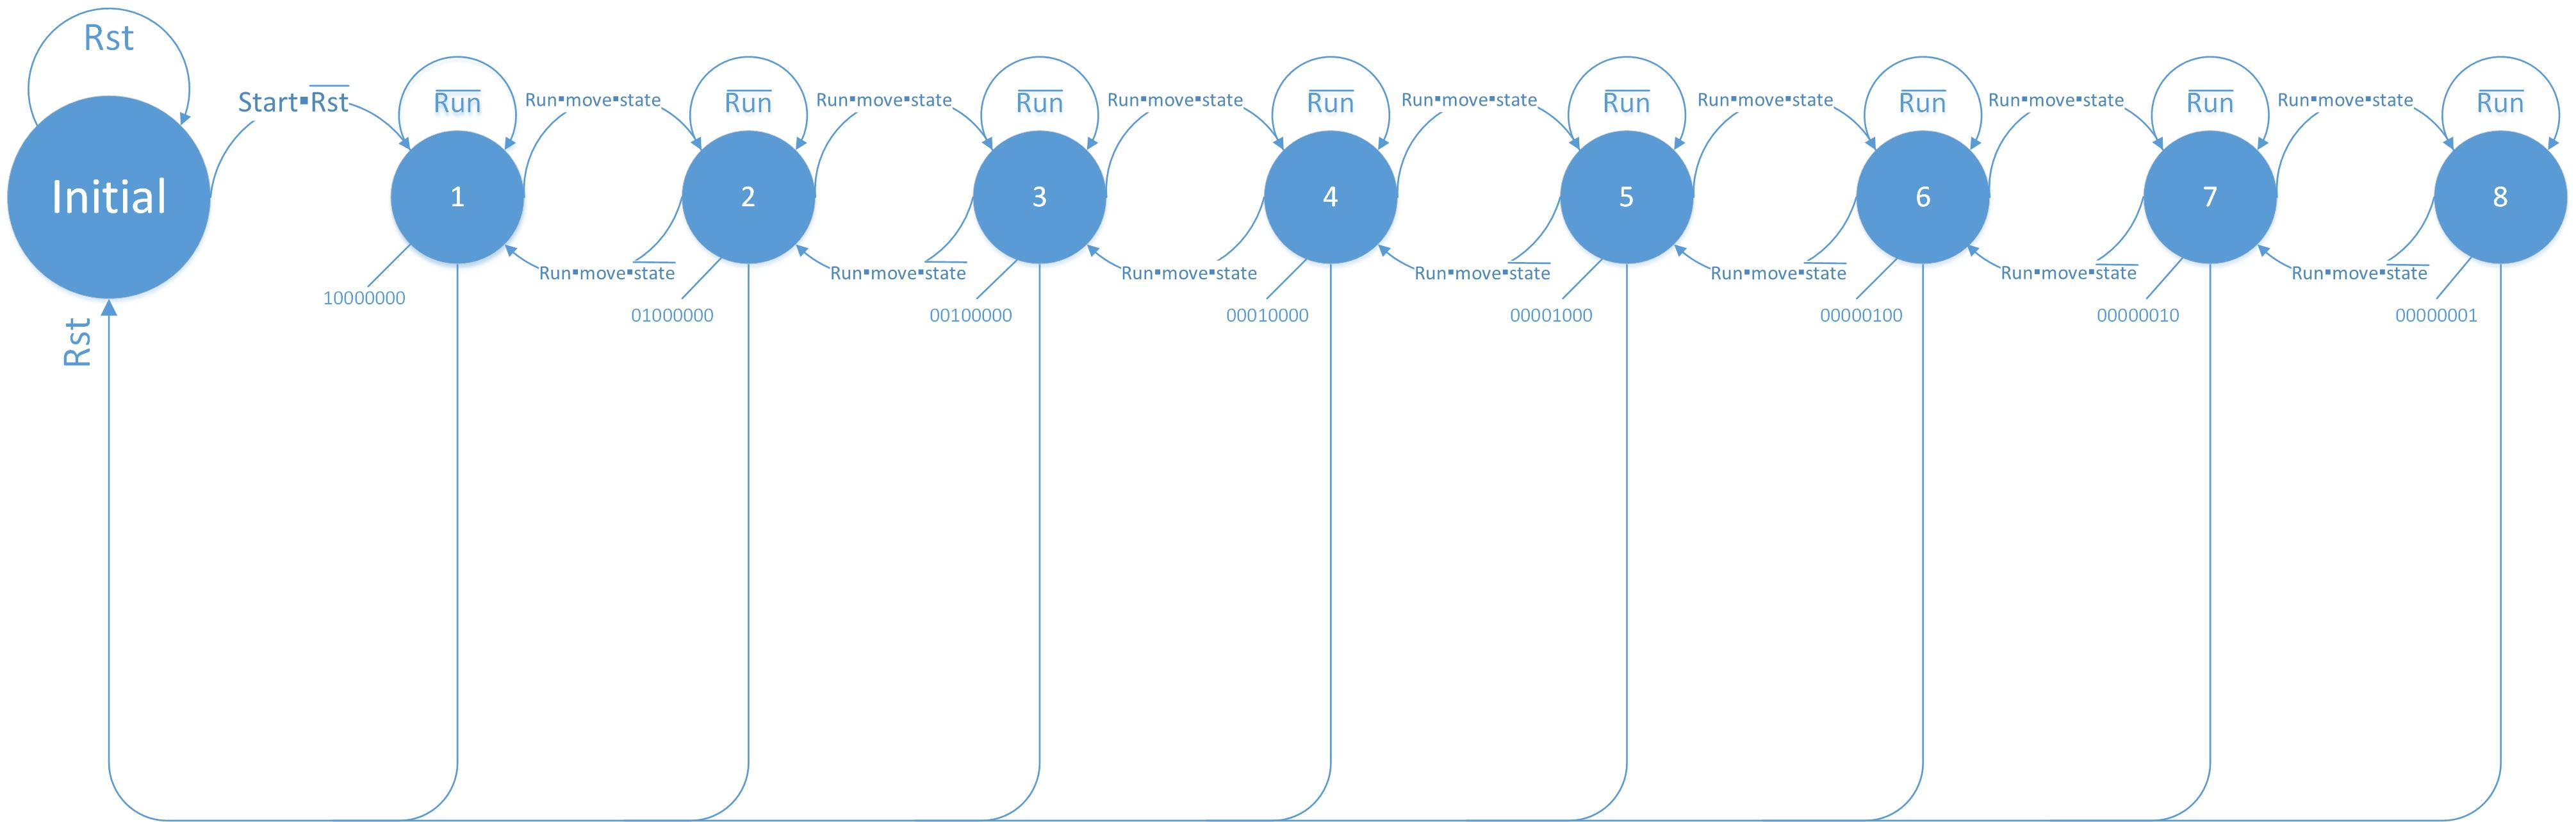
\includegraphics[scale=0.2]{状态机图.jpg}
    \caption{状态机图}
    \label{FIG.4}
\end{figure}
\subsection{程序实现}

见附件中代码。

\subsection{仿真与测试}
\subsubsection{各模块RTL图}

见图\ref{FIG.5}、\ref{FIG.6}、\ref{FIG.7}、
\ref{FIG.8}、\ref{FIG.9}。
\begin{figure}[H]

    \centering
    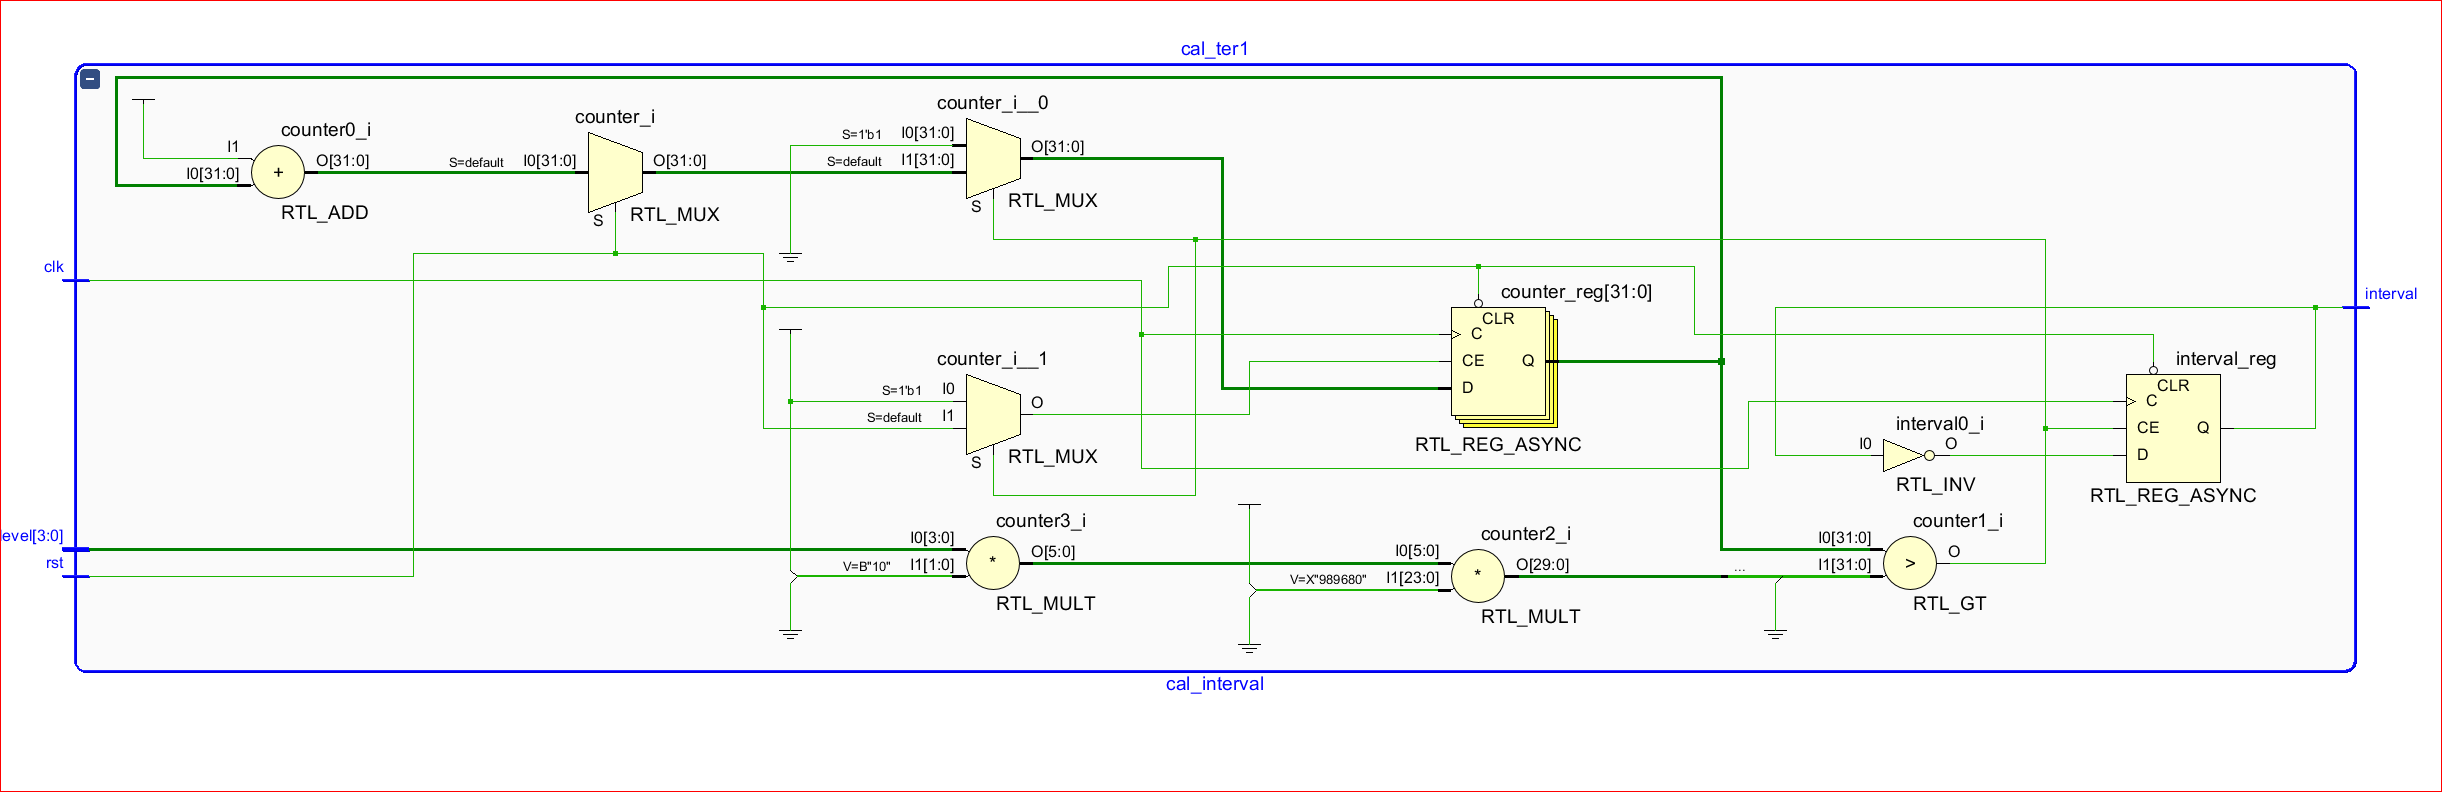
\includegraphics[width=\linewidth]{cal_interval.PNG}
    \caption{cal interval}
    \label{FIG.5}
\end{figure}

\begin{figure}[H]
    \centering
    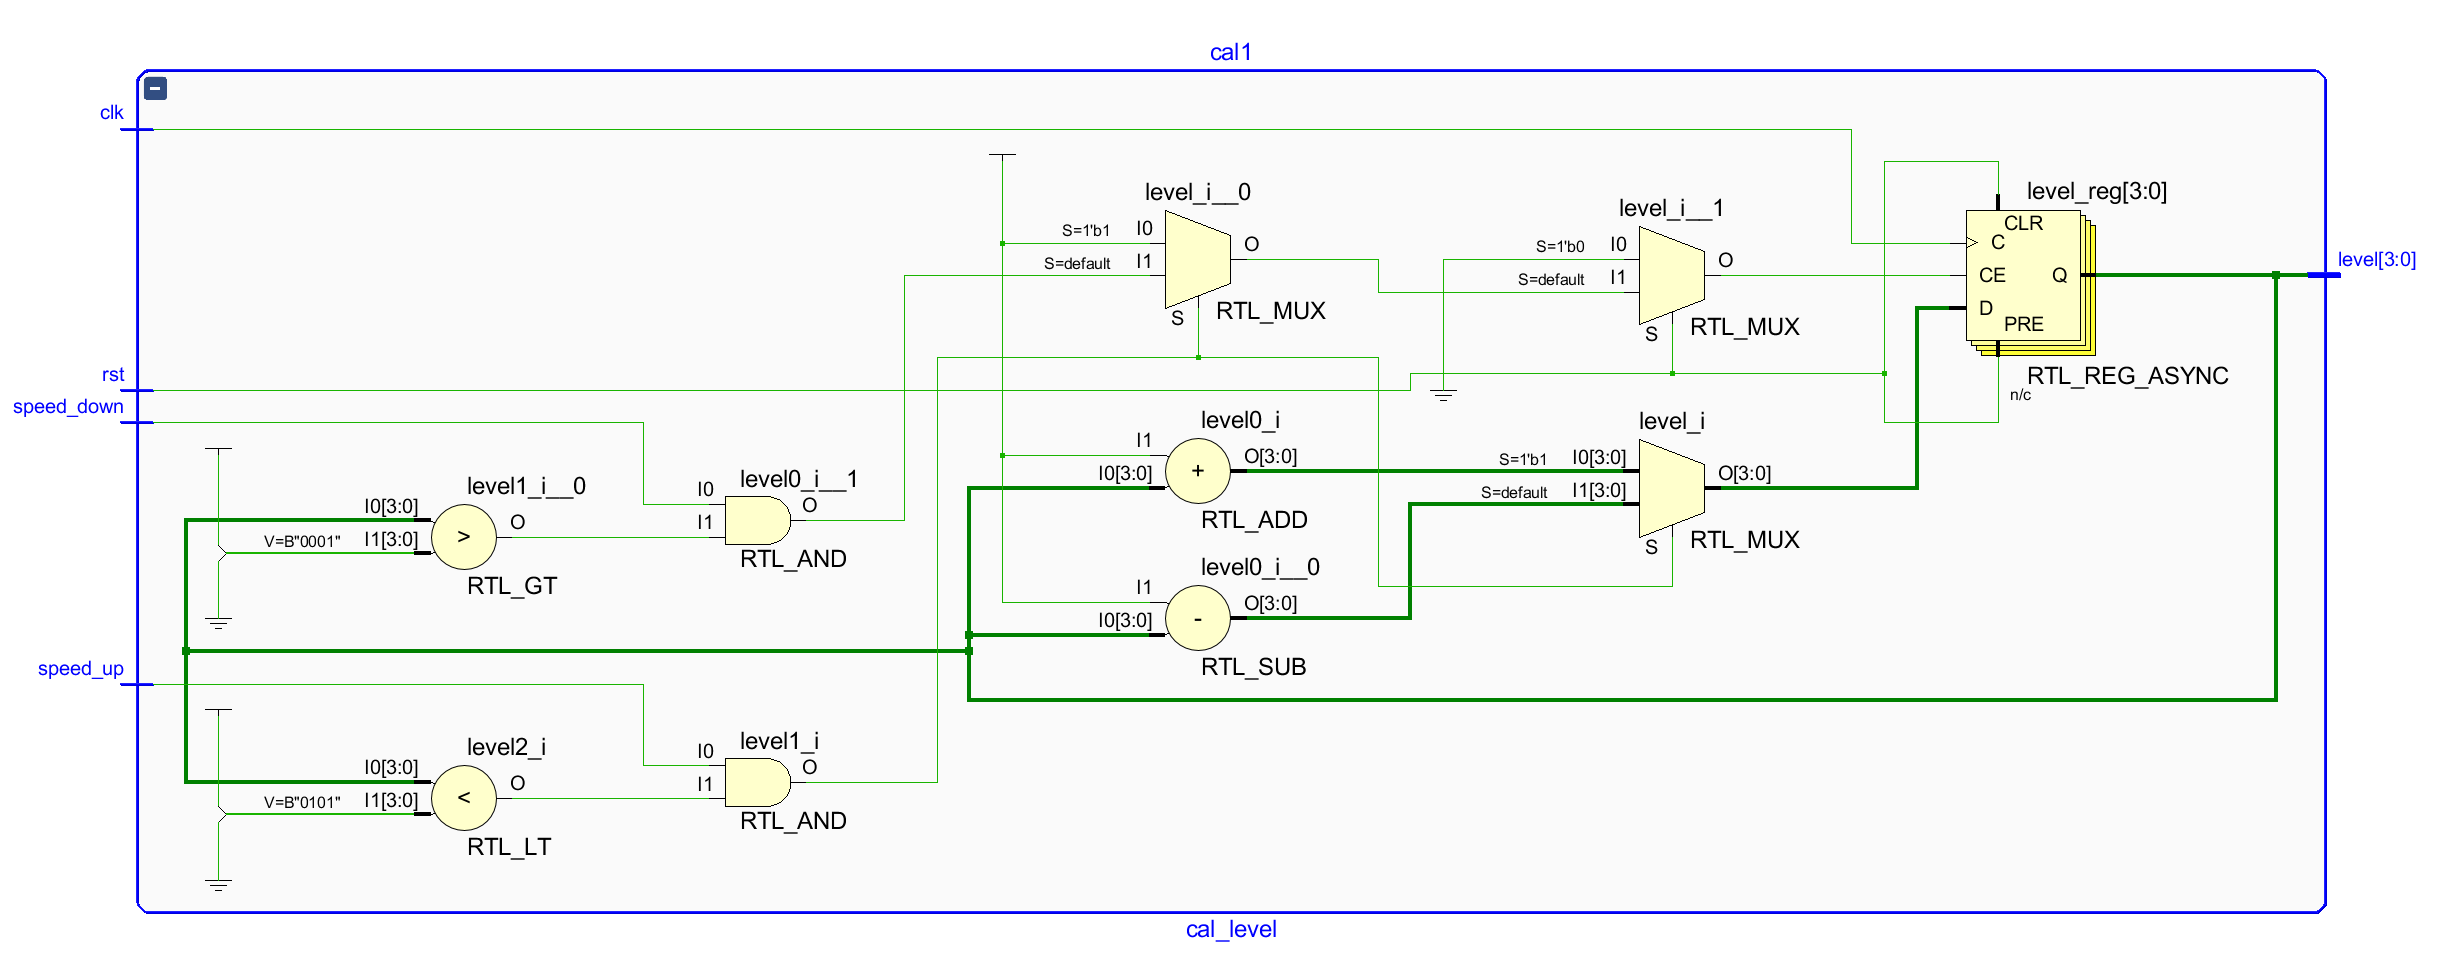
\includegraphics[width=\linewidth]{cal_level.PNG}
    \caption{cal level}
    \label{FIG.6}
\end{figure}

\begin{figure}[H]
    \centering
    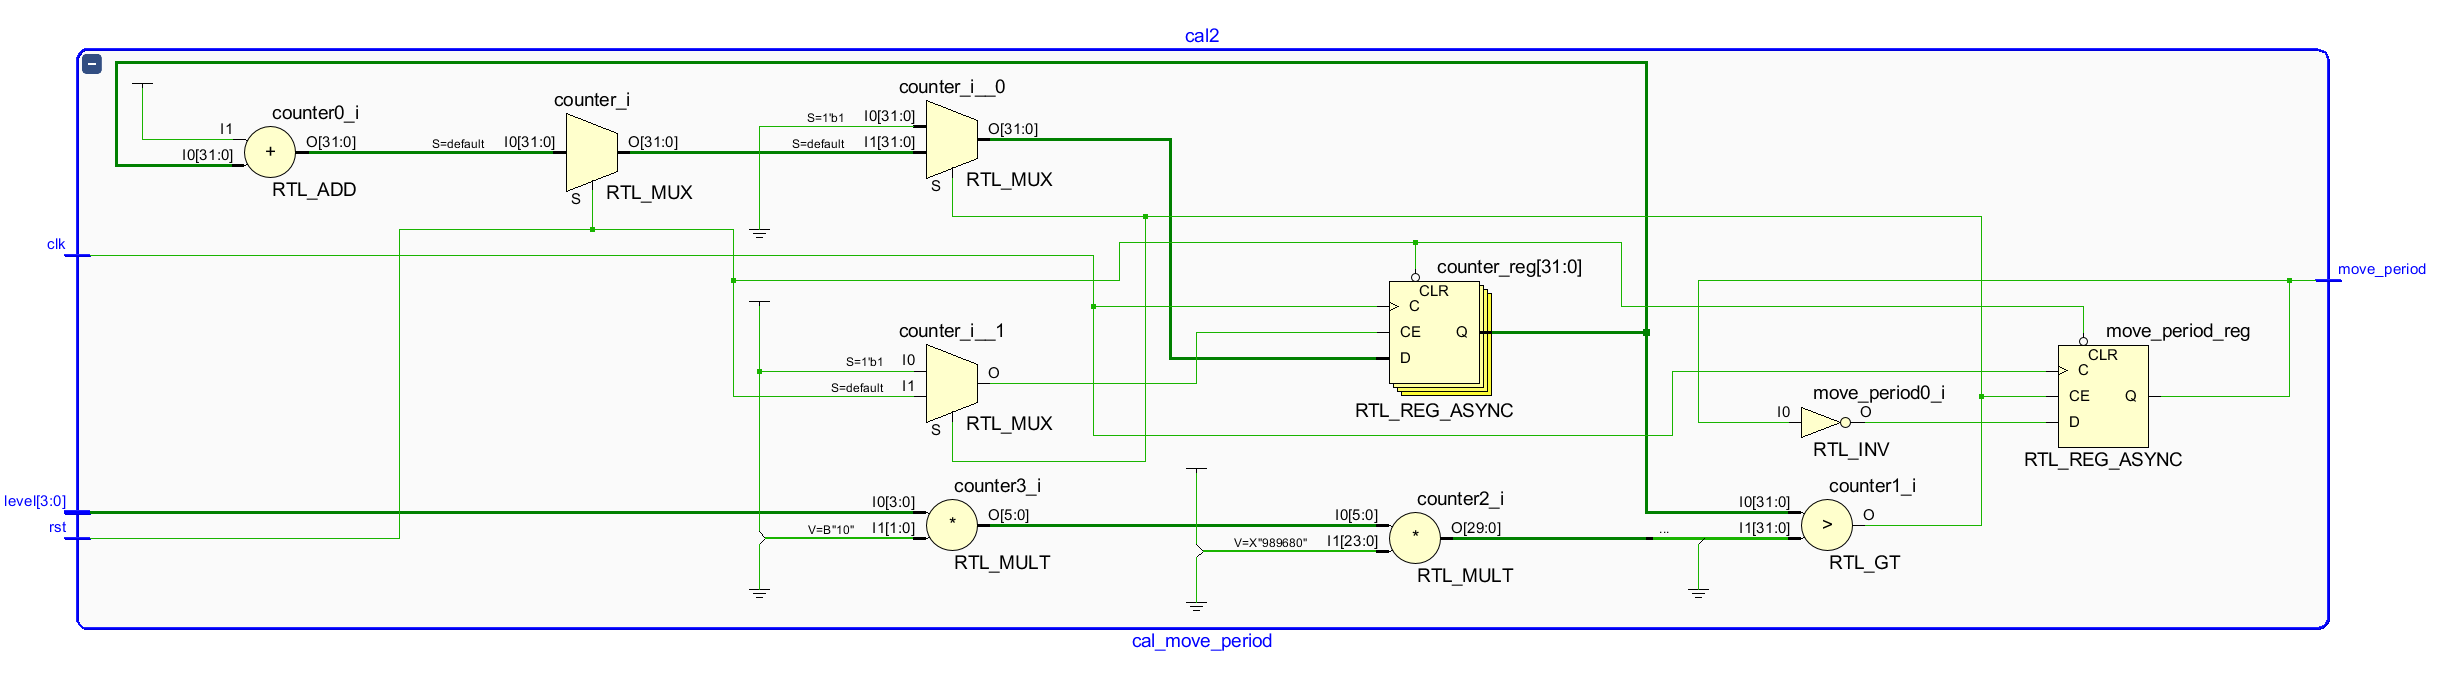
\includegraphics[width=\linewidth]{cal_move_period.PNG}
    \caption{cal move period}
    \label{FIG.7}
\end{figure}

\begin{figure}[H]
    \centering
    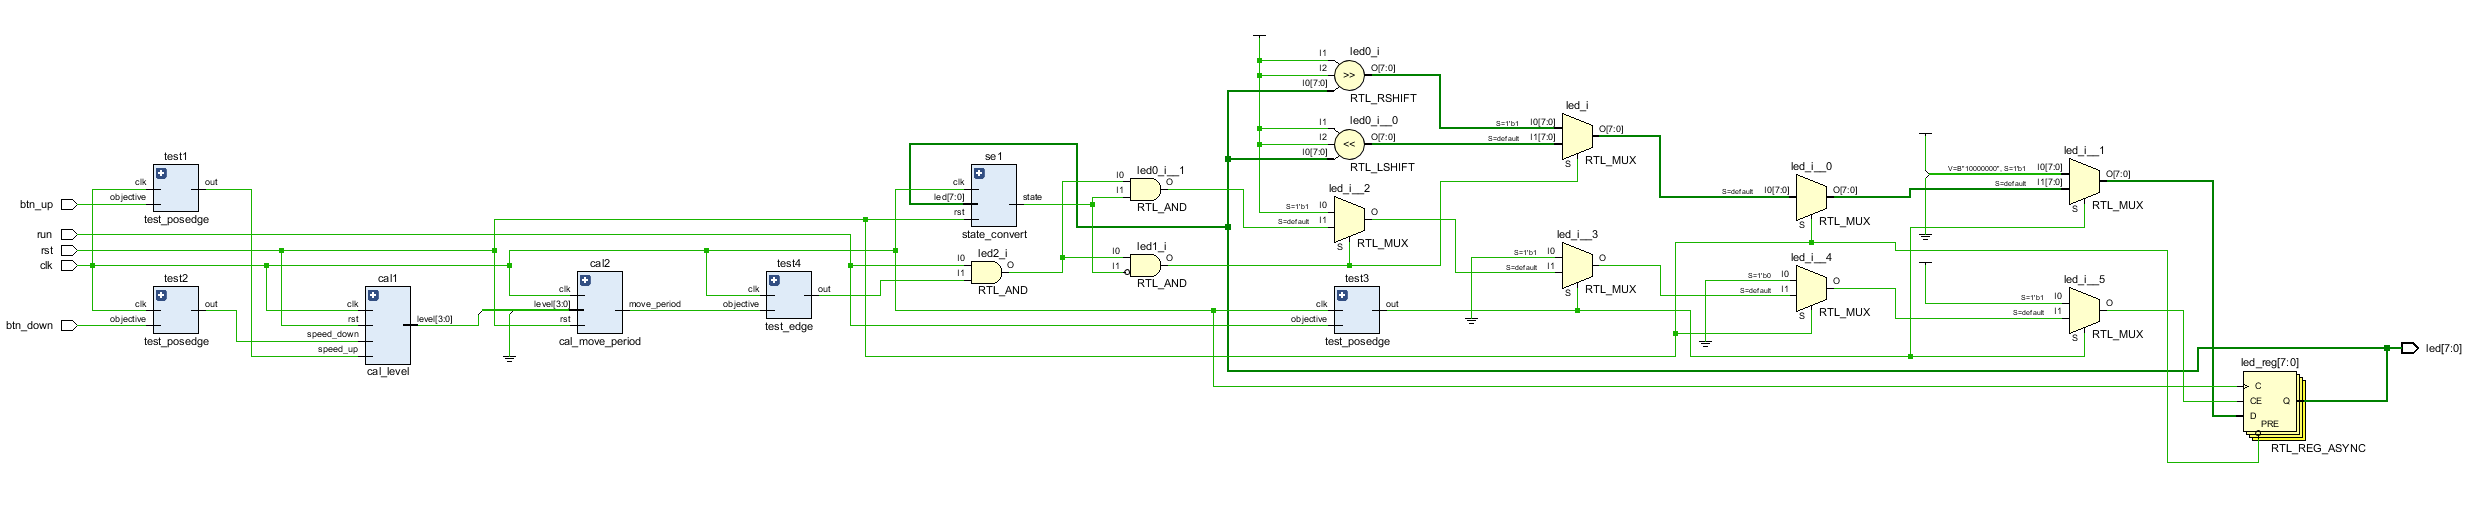
\includegraphics[width=\linewidth]{overall.PNG}
    \caption{overall}
    \label{FIG.8}
\end{figure}

\begin{figure}[H]
    \centering
    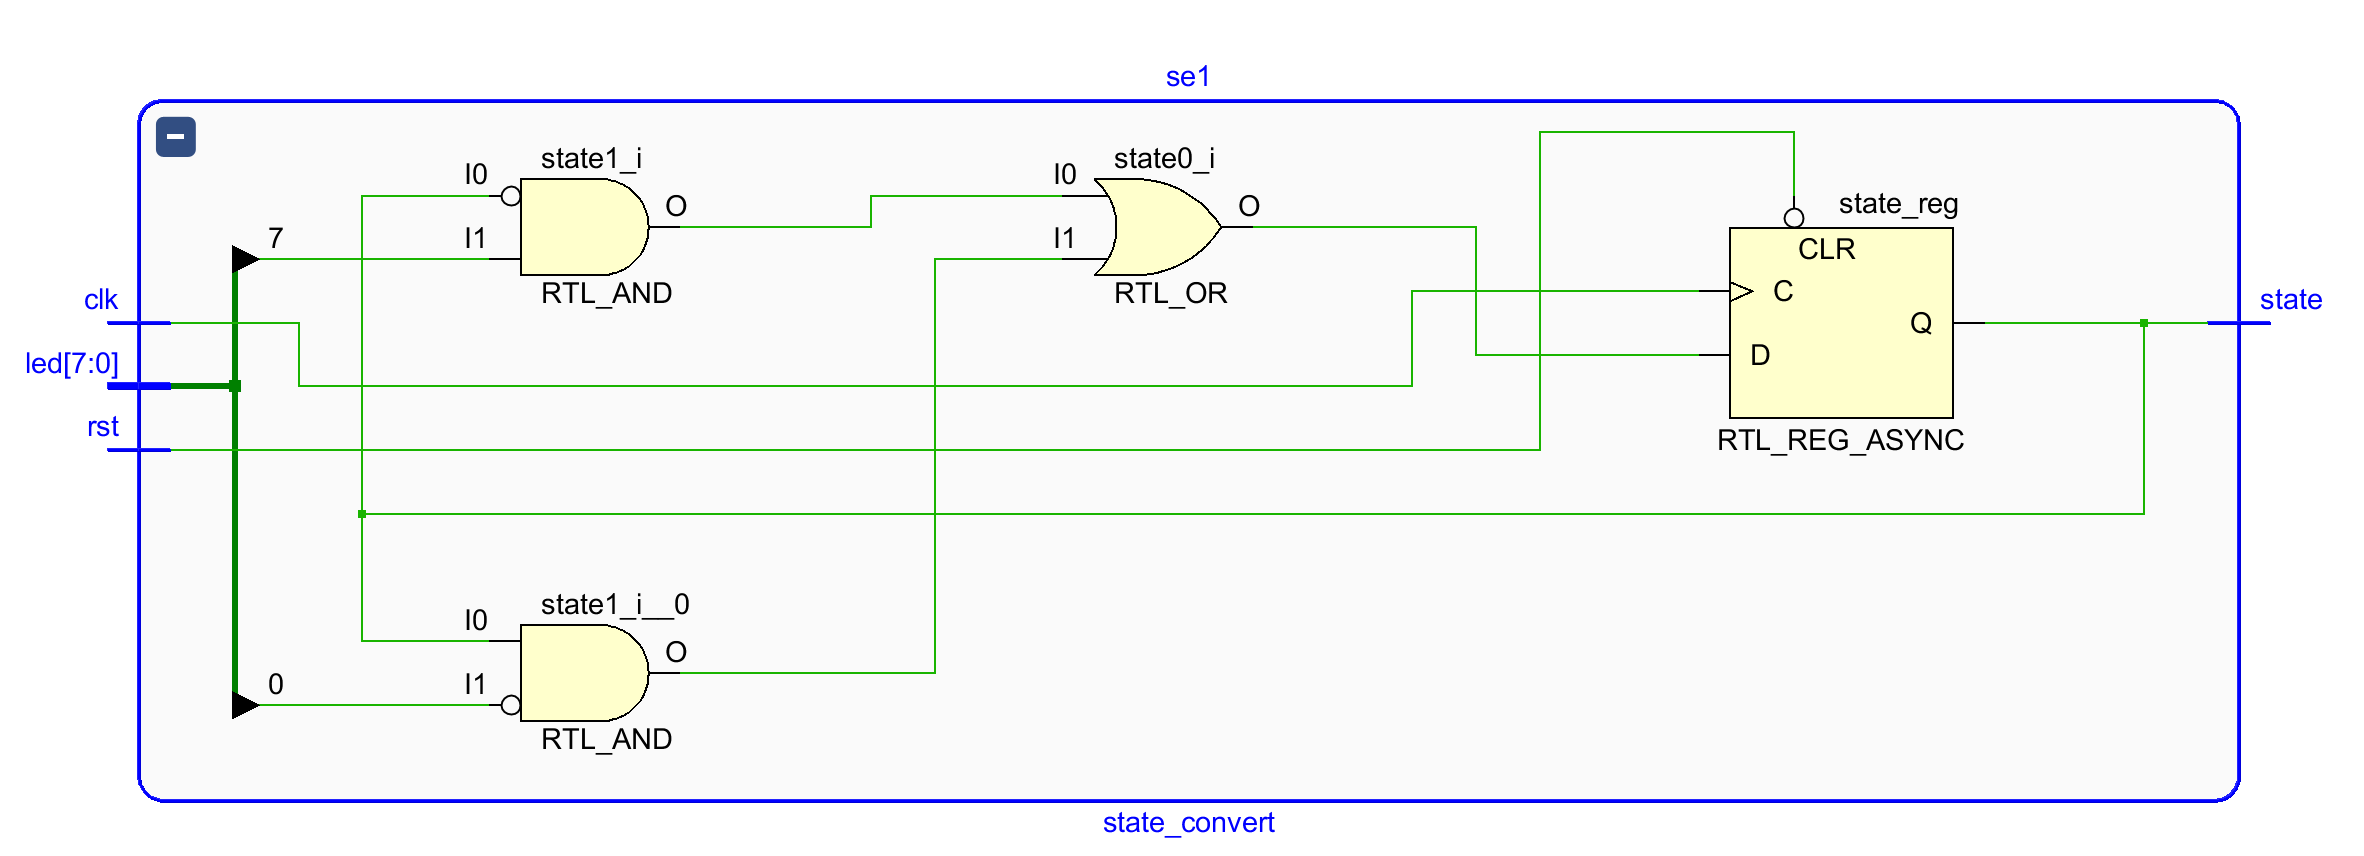
\includegraphics[width=\linewidth]{state_convert.PNG}
    \caption{state convert}
    \label{FIG.9}
\end{figure}
\subsubsection{测试}

见图\ref{FIG.10}、\ref{FIG.11}。

\begin{figure}[H]
    \centering
    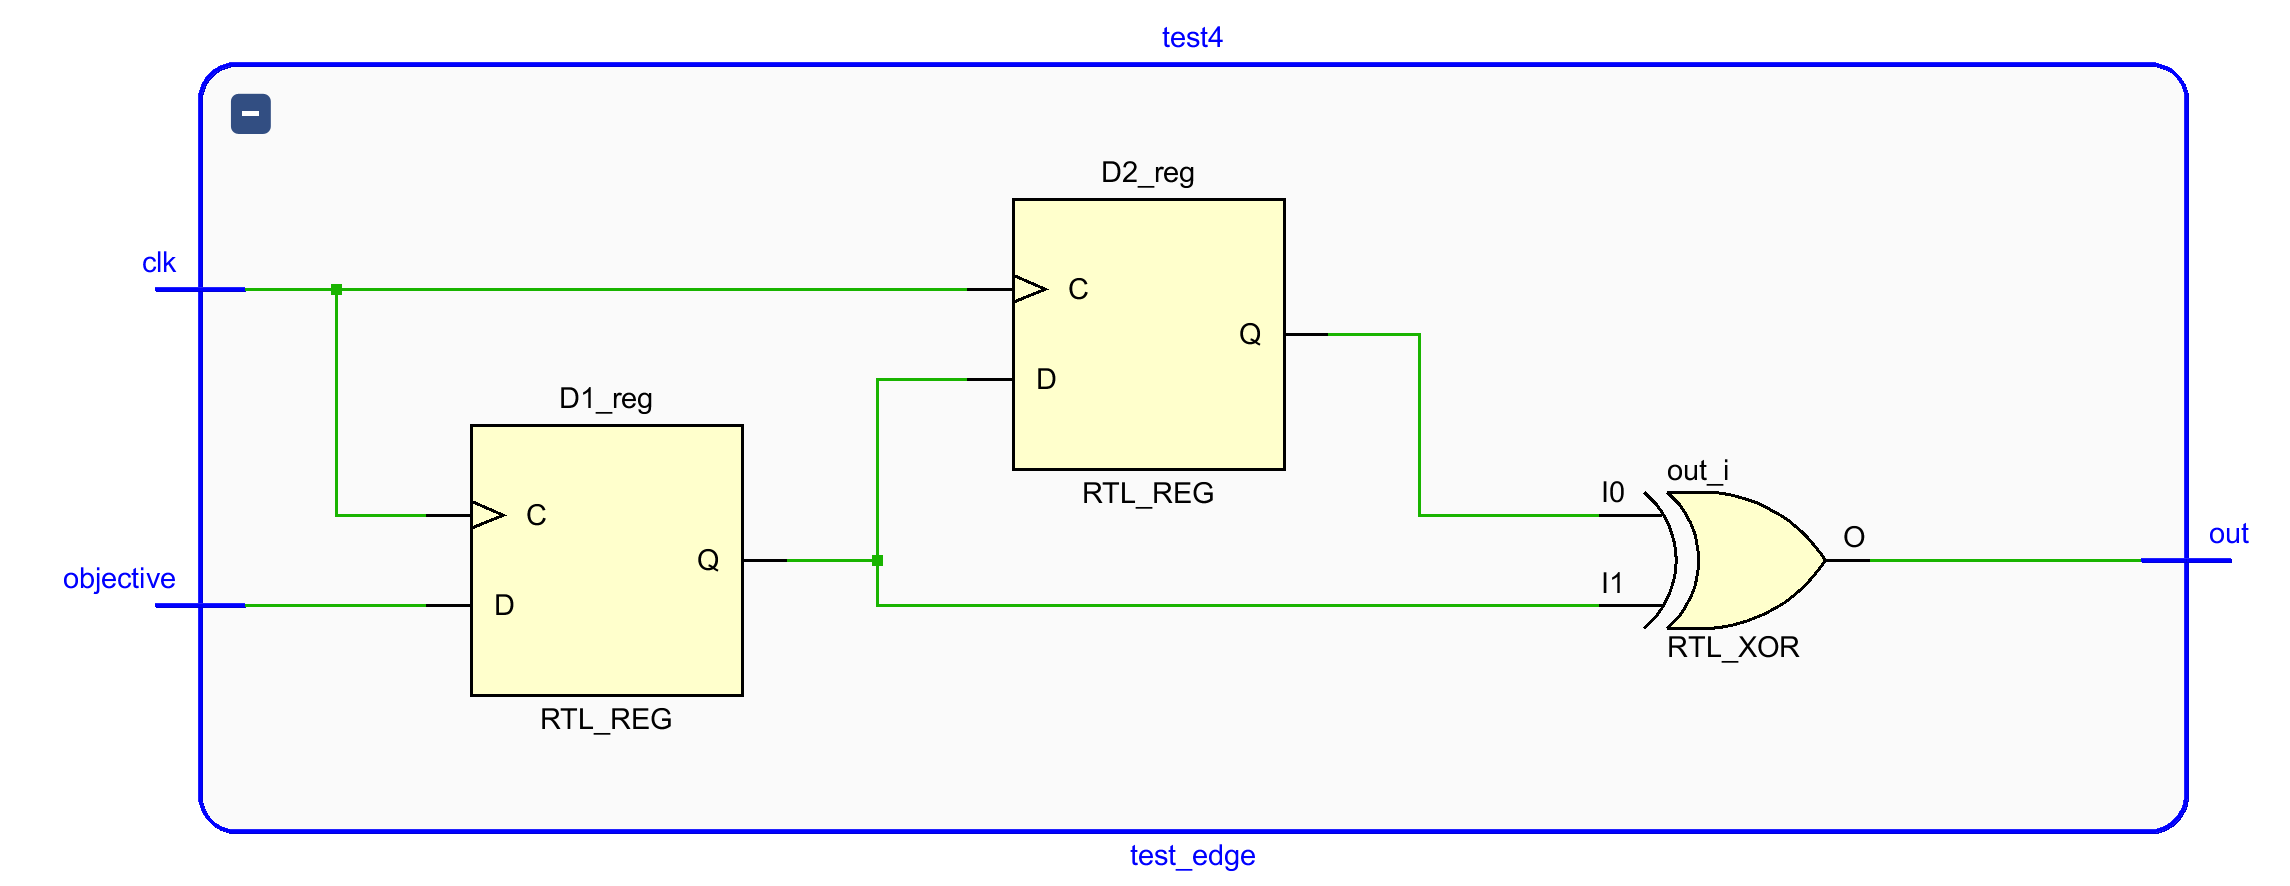
\includegraphics[width=\linewidth]{test_edge.PNG}
    \caption{test edge}
    \label{FIG.10}
\end{figure}
\begin{figure}[H]
    \centering
    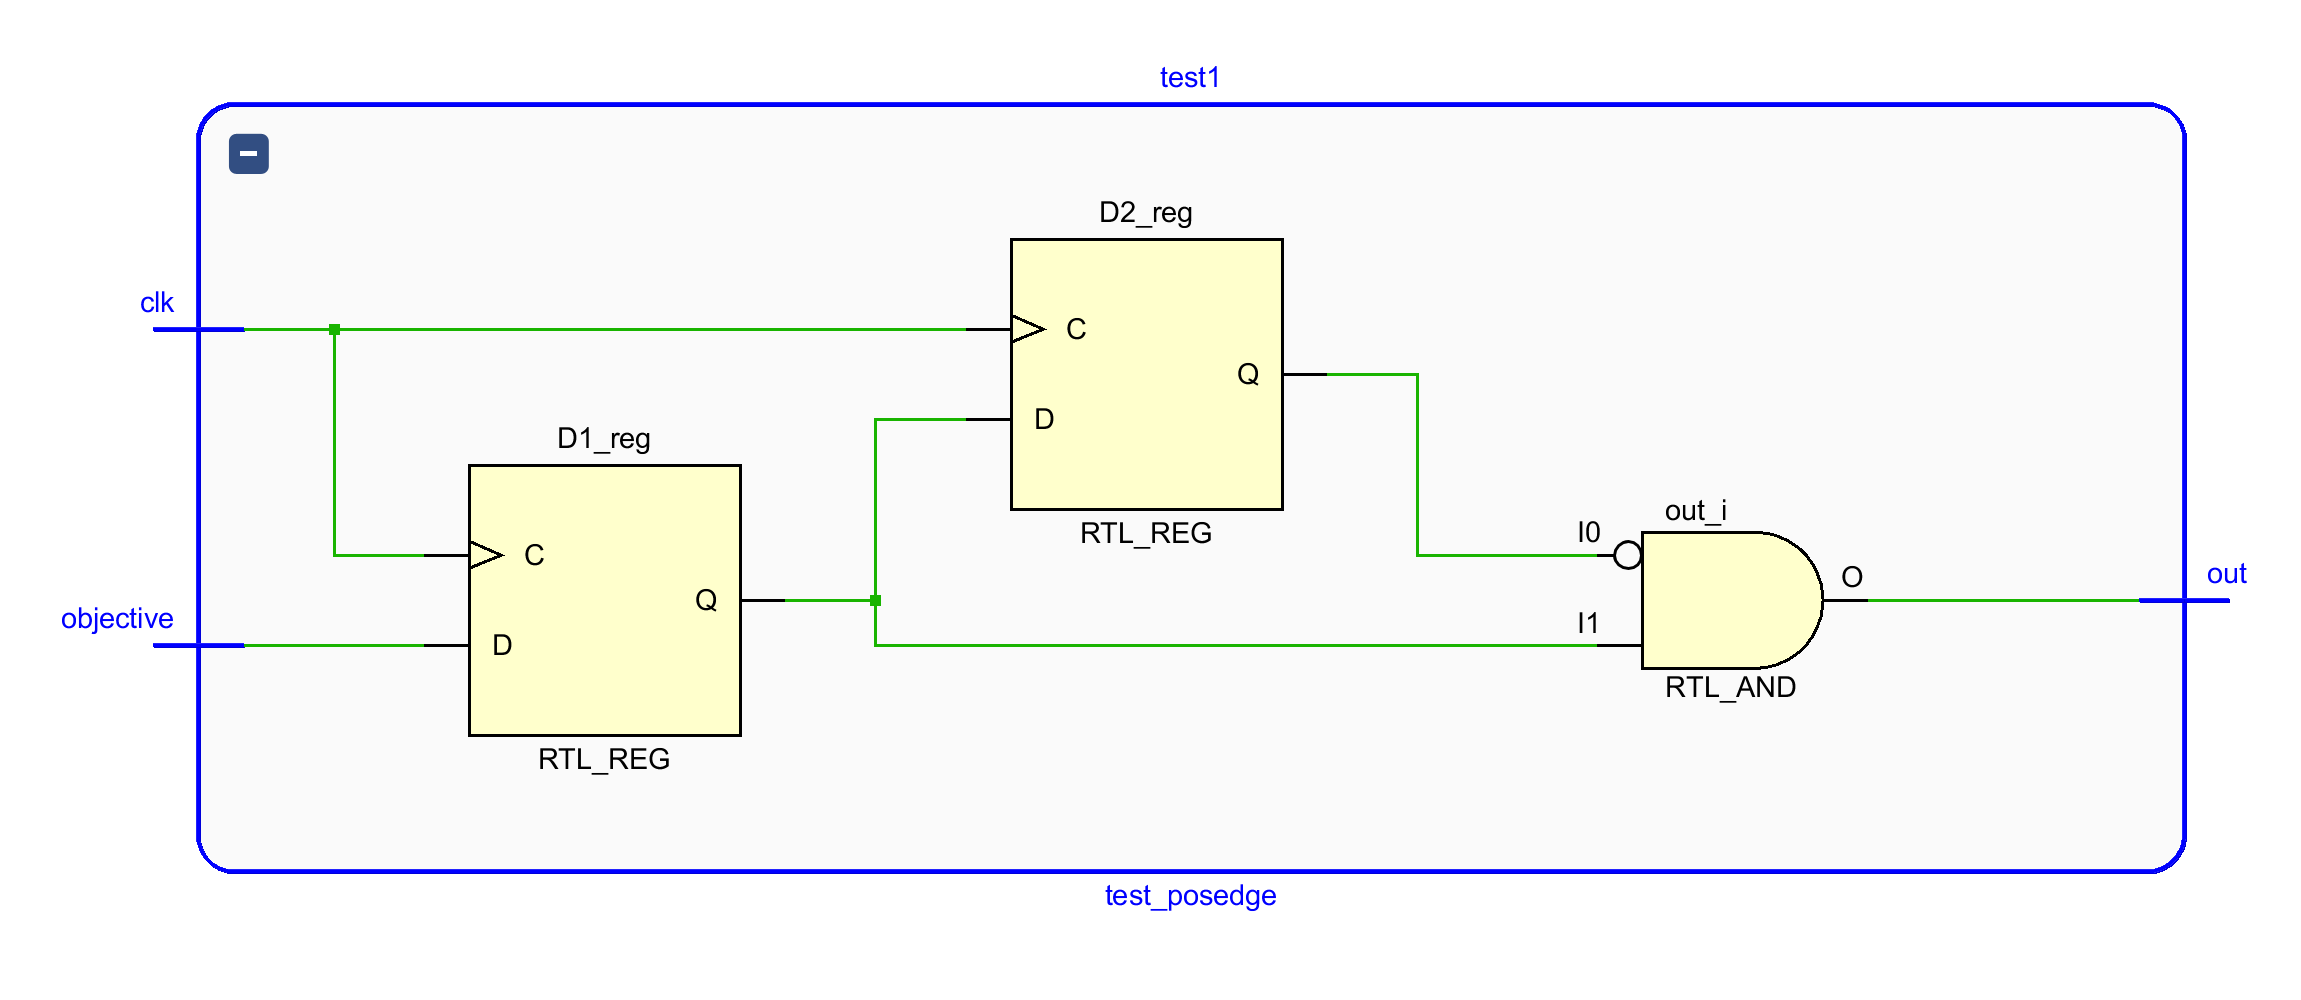
\includegraphics[width=\linewidth]{test_posedge.PNG}
    \caption{test posedge}
    \label{FIG.11}
\end{figure}
\subsection{综合与实现}
\subsection{生成mcs文件烧录到flash}
\subsection{运行结果显示}
按照预期成功运行。

按下开关时,流水灯从左向右滚动,抵达最右侧时再从右向左滚动。
同时可以利用上下两个开关调整流水灯的滚动速度,实现变速流水灯。

\section{遇到的问题及解决方法}
\subsection{Ambiguous clock in event control}

\href{https://stackoverflow.com/questions/27145548/ambiguous-clock-in-event-control}{ambiguous-clock-in-event-control} 

问题原因: 

一个时序电路always语句块里可能有两个条件同时满足比如
    if A则B
    if C则D
AC可能同时为真则可能进入两个逻辑之中

\subsection{stimulation error}
问题原因:

模块实例化时只能用wire类型接受参数,可以用wire类型和reg类型传递参数。

\begin{figure}[H]
    \centering
    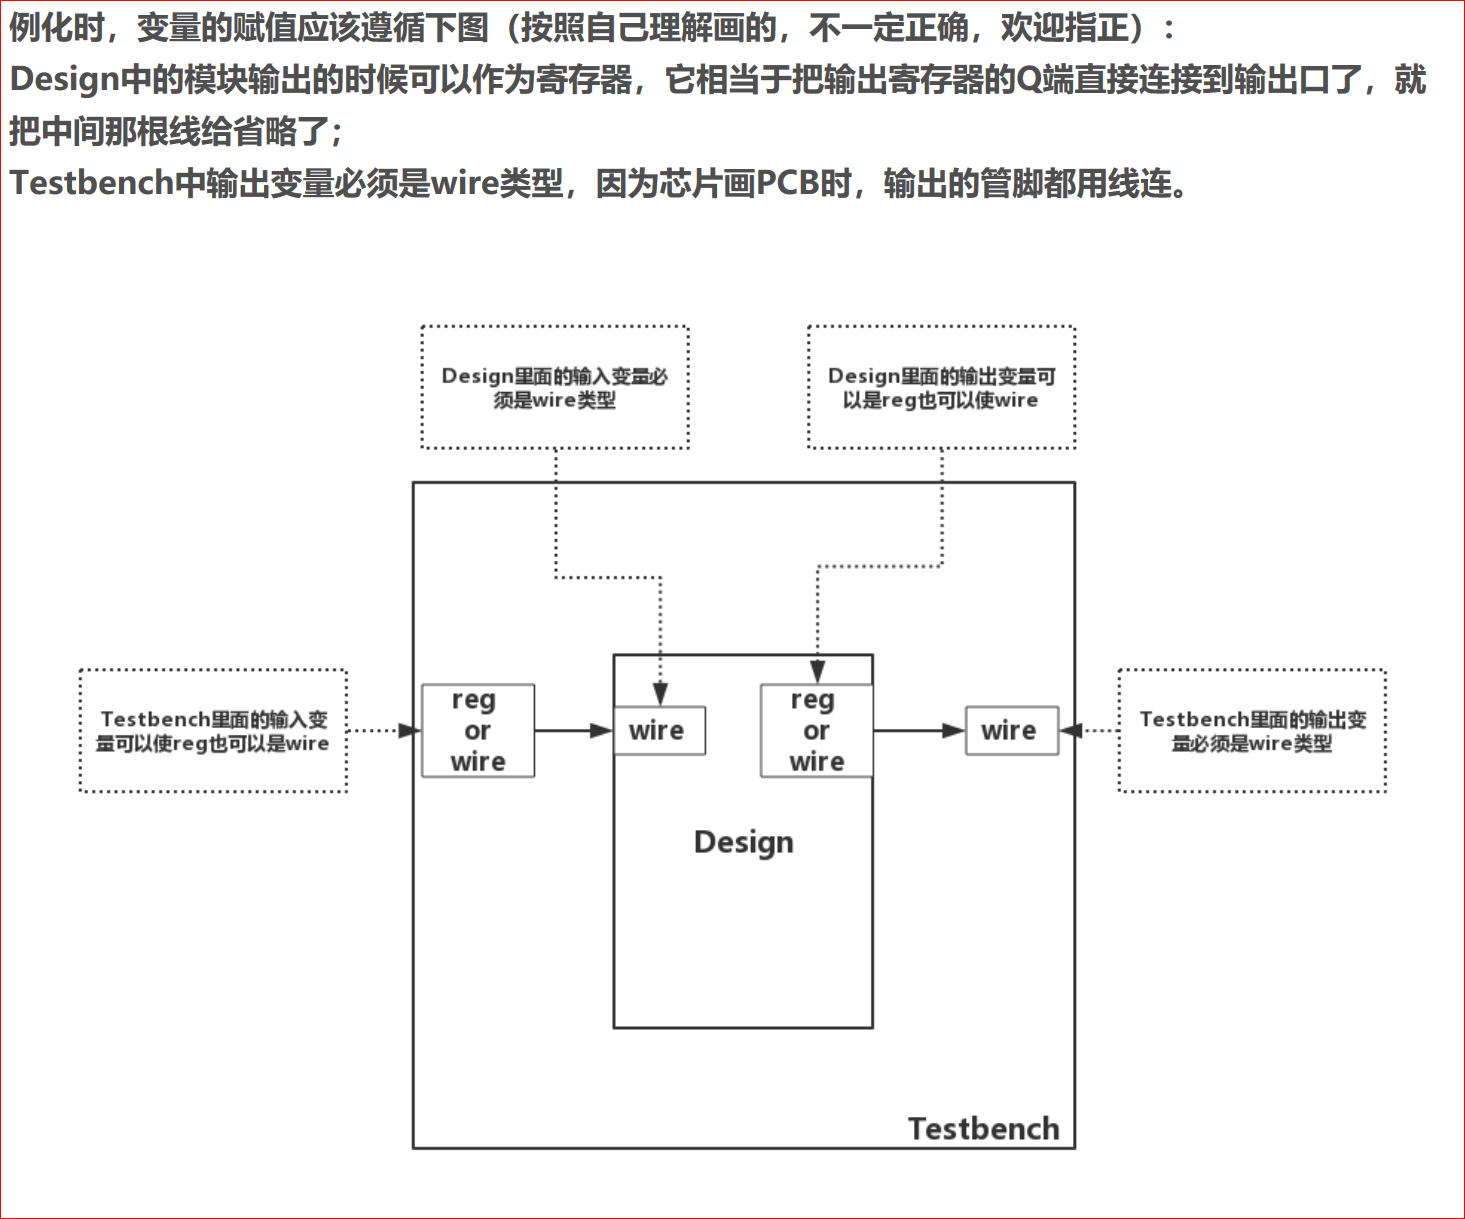
\includegraphics[width=\linewidth]{0.PNG}
    \caption{原因分析}
    \label{FIG.12}
\end{figure}

\subsection{时钟分频与仿真}
问题原因: 

仿真时可用频率远高于所需时钟频率,
需修改程序后方可仿真否则综合实现后频率过高无法察觉灯闪烁移动
\section{小组成员分工}

王聚海
\begin{itemize}
    \item 循环流水灯设计、实现、测试、上板
    \item 文档撰写
\end{itemize}

冯开宇
\begin{itemize}
    \item 文档撰写和排版
\end{itemize}

\end{document}
